% Standard LaTeX document template
%  BE SURE TO PROCESS DOCUMENT TWICE IF IT CONTAINS CROSS-REFERENCES!

\documentclass[12pt]{article}
\usepackage[round]{natbib} %allow to set the bibliography style and
% import the bibliography file. See Bibliography management with
% natbib for more information on
% https://www.sharelatex.com/learn/Bibliography_management_with_natbib.
% See the reference sheet for natbib on
% http://merkel.zoneo.net/Latex/natbib.php.
% Several .bst files can be
% downloaded from http://kinglab.eeb.lsa.umich.edu/pub/biblios/bst/

\usepackage{graphicx,epsfig}
\usepackage{amssymb,amsmath,amsfonts,bm,color,supertabular,longtable,multirow}
\usepackage[colorlinks=true,linkcolor=black,citecolor=black,urlcolor=black]{hyperref}

\setlength{\oddsidemargin}{0in} % left margin, odd pages
\setlength{\evensidemargin}{0in} % left margin, even pages
\setlength{\textwidth}{6.5in} % widtth of text on page
\setlength{\topmargin}{-.3in} % add to default 1 in
\setlength{\headsep}{0in}     % add to default 25pt
\setlength{\textheight}{8.7in}  % height of text on page
\setlength{\parskip}{.1in}            % vertical space between paragraphs
\setcounter{tocdepth}{2}

%\setlength{\parindent}{0in}            % amount of indentation of paragraph


%  newcommands -- more newcommands used in the document.
%  not just in the preamble

\newcommand{\Var}{\mbox{Var}}
\newcommand{\Cov}{\mbox{Cov}}
\newcommand{\E}{\mbox{E}}
\newcommand{\ubeta}{\mbox{\boldmath$\beta$}}
% Independence symbol
\newcommand\independent{\protect\mathpalette{\protect\independenT}{\perp}}
\def\independenT#1#2{\mathrel{\rlap{$#1#2$}\mkern2mu{#1#2}}}


\title{STAT 501 Case Study Assignment} 
\author{Quan Zhao\\
School of Mathematics and Statistics\\ Victoria University of Wellington, New Zealand} 
%\date{}  % Add \date{} to make a blank date.


%  main body of document

\begin{document}

% Titlepage
\maketitle

\begin{abstract}
  This study delves into the intricate relationship between students' interest and aptitude in science and the overall development of their respective countries, using data from the Programme for International Student Assessment (PISA) and the Human Development Index (HDI). Through correlation and regression analyses of data from 54 countries, we found that higher Human Development and income levels do not necessarily translate to increased support or interest in science. Specifically, countries with lower HDI values tend to exhibit a stronger interest in science. The Netherlands, despite its economic prosperity, offers comparatively lower support for science, while Finland, with its high HDI, displays reduced student interest in the subject. These findings challenge the prevailing assumption that affluence and development invariably foster greater support and interest in science. The study underscores the need for individual countries, especially those like the Netherlands and Finland, to re-evaluate their science education strategies and funding mechanisms. Future research is recommended to explore the cultural and societal nuances influencing these trends.
\end{abstract}


% % Table of Contents
% \tableofcontents


% \setlength{\baselineskip}{0.25in} % min space from bottom of one line

%                                  % to top of next in a paragraph

%                                  % place after \begin{document}



% \newpage  % start from a new page
\section{Introduction}

\label{s.intro}

The relationship between students' interest and aptitude in science and the overall development of countries on a global scale is a subject that is both fascinating and deserving of in-depth analysis. Understanding this relationship can offer valuable insights into the educational, economic, and social fabric of nations.

In this comprehensive study, we aim to shed light on this complex issue by conducting a rigorous statistical analysis at the national level. To achieve this, we have integrated multiple data sources, including the Programme for International Student Assessment (PISA) \cite{oecd_pisa_2016} and the Human Development Index (HDI) \cite{undp_hdi_2021} from United Nations data. PISA provides a robust measure of 15-year-old students' science literacy, while the HDI offers a composite index of life expectancy, education, and per capita income indicators, which are used to rank countries into tiers of human development.

Our primary objective is to offer a high-level overview that elucidates the relationship between students' scientific capabilities and interests and their country's level of development. By doing so, we aim to identify key issues that may be hindering progress in both educational and developmental sectors. Furthermore, our analysis serves as a foundation for proposing actionable solutions that could be implemented to improve educational outcomes and, by extension, the overall well-being of nations.

Through this study, we hope to contribute to the ongoing discourse on education and development, providing policymakers, educators, and stakeholders with valuable data and insights that can guide future initiatives and reforms.

% Context and background information.
% \cite{Liu05}

% \section{Objectives and Scope}

% %Specific objectives of the statistical consultation.
% %Scope of the analysis including what is and is not covered.

% \begin{itemize}
%   \item Identify the top ten countries in overall sciences scores.
%   \item Determine whether wealthier (higher income) countries tend to provide more support.
%   \item Determine whether students from countries with a higher HDI show more interest in science.
%   \item Determine whether the level of support and interest have an effect on overall science scores.
% \end{itemize}

\section{Objectives and Scope}

\label{s.objectives}

This study aims to provide a comprehensive understanding of the relationship between students' interest and aptitude in science and the overall development of their respective countries. To achieve this, we have outlined the following specific objectives:

\begin{itemize}
\item \textbf{Science Literacy Rankings:} Identify the top ten countries with the highest overall science scores based on PISA assessments. This will serve as a benchmark for evaluating the effectiveness of educational systems in fostering scientific literacy.

\item \textbf{Wealth and Educational Support:} Investigate whether countries with higher per capita income levels tend to provide more educational support in science. Support could be measured in terms of educational funding, availability of science programs, and teacher-to-student ratios.

\item \textbf{Human Development and Scientific Interest:} Examine the correlation between a country's Human Development Index (HDI) and the level of interest in science among its students. Interest could be gauged through survey data, extracurricular participation, or other relevant metrics.

\item \textbf{Impact of Support and Interest:} Assess whether the level of educational support and student interest in science have a significant impact on overall science scores. This will involve multivariate statistical analyses to control for other influencing factors.
\end{itemize}

\textbf{Scope of Analysis:}

The scope of this study is limited to:

\begin{itemize}
\item Data from the most recent PISA assessments, focusing on 15-year-old students' performance in science.

\item HDI data from the United Nations, specifically examining the components related to education and income.

\item Countries for which both PISA and HDI data are available, to ensure a comprehensive and comparative analysis.
\end{itemize}

This study will not cover:

\begin{itemize}
\item In-depth analyses of individual educational systems or curricula.

\item Factors such as cultural attitudes or government policies, unless they are directly related to educational support or student interest in science.
\end{itemize}

By adhering to these objectives and scope, we aim to provide a robust analysis that can inform policy decisions and educational reforms aimed at improving both educational outcomes and national development.

% \section{Methodology}

% Overview of the statistical methods used.
% Software and tools used for analysis.

\section{Data Description}

\subsection{Programme for International Student Assessment (PISA)}

The Programme for International Student Assessment (PISA) is an initiative by the OECD to evaluate the knowledge and skills of 15-year-old students worldwide. PISA assesses the ability of these students to apply their reading, mathematics, and science knowledge to real-world challenges.

In our analysis, we have incorporated several metrics from PISA, including:
\begin{itemize}
\item Overall Science Score: This represents the average score of 15-year-olds in science.
\item Interest in Science: A measure of students' enthusiasm and curiosity towards scientific topics.
\item Support for Scientific Inquiry: This metric gauges the encouragement and resources provided to students for exploring scientific concepts.
\end{itemize}

\subsection{Human Development Index (HDI)}

The Human Development Index (HDI) is a composite measure designed to evaluate long-term progress in three fundamental dimensions of human development:
\begin{itemize}
\item A long and healthy life.
\item Access to knowledge.
\item A decent standard of living.
\end{itemize}

For the purpose of this study, we have incorporated the following components from the HDI:
\begin{itemize}
\item Income Index: Represents the economic capability of individuals in a country.
\item Health Index: A measure of the overall health and longevity of the population.
\item Education Index: Evaluates the access to and quality of education in a country.
\item Overall Human Development Index: The composite score that combines all the above dimensions.
\end{itemize}


\subsection{Data Imputation}
\label{ss.imputation}

Figure $\ref{fig:missing}$ (a) illustrates the presence of missing data in our initial dataset. Given that there is no direct correlation between PISA and HDI data, we opted to exclude rows where either all PISA-related information or all HDI-related information was absent.

Following this filtration process, Figure $\ref{fig:missing}$ (b) presents the status of the dataset with respect to missing values. Post-filtering, we retained data for 54 countries.

To address the remaining missing values, we employed the "predictive mean matching" (PMM) method from the R MICE package \cite{mice_package}. This approach allows for a more robust imputation by leveraging the relationships between variables to predict missing values.


\begin{figure}[htb]
  \begin{minipage}[b]{1.0\linewidth}
    \centering
    \centerline{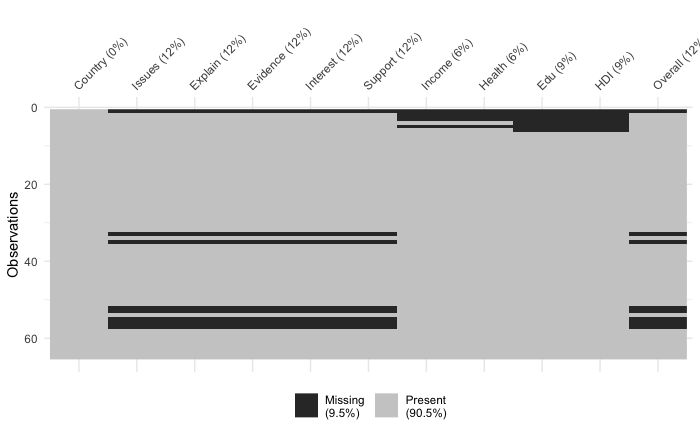
\includegraphics[width=10.0cm]{images/null_1}}
  %  \vspace{1.5cm}
    \centerline{(a) raw data}\medskip
  \end{minipage}
  \hfill
  \begin{minipage}[b]{1.0\linewidth}
    \centering
    \centerline{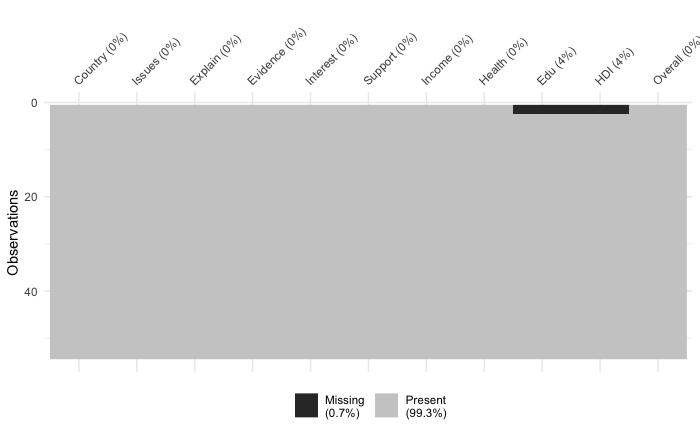
\includegraphics[width=10.0cm]{images/null_2}}
  %  \vspace{1.5cm}
    \centerline{(b) remove missing }\medskip
  \end{minipage}
  %
  \caption{Visualize Missing Data}
  \label{fig:missing}
  %
  \end{figure}

  \subsection{Top 10 Countries in PISA Overall}
  \label{ss.top10}

  Fig $\ref{fig:top10}$ shows the 10 highest PISA overall score countries.

  \begin{figure}[htb]
    \centering
    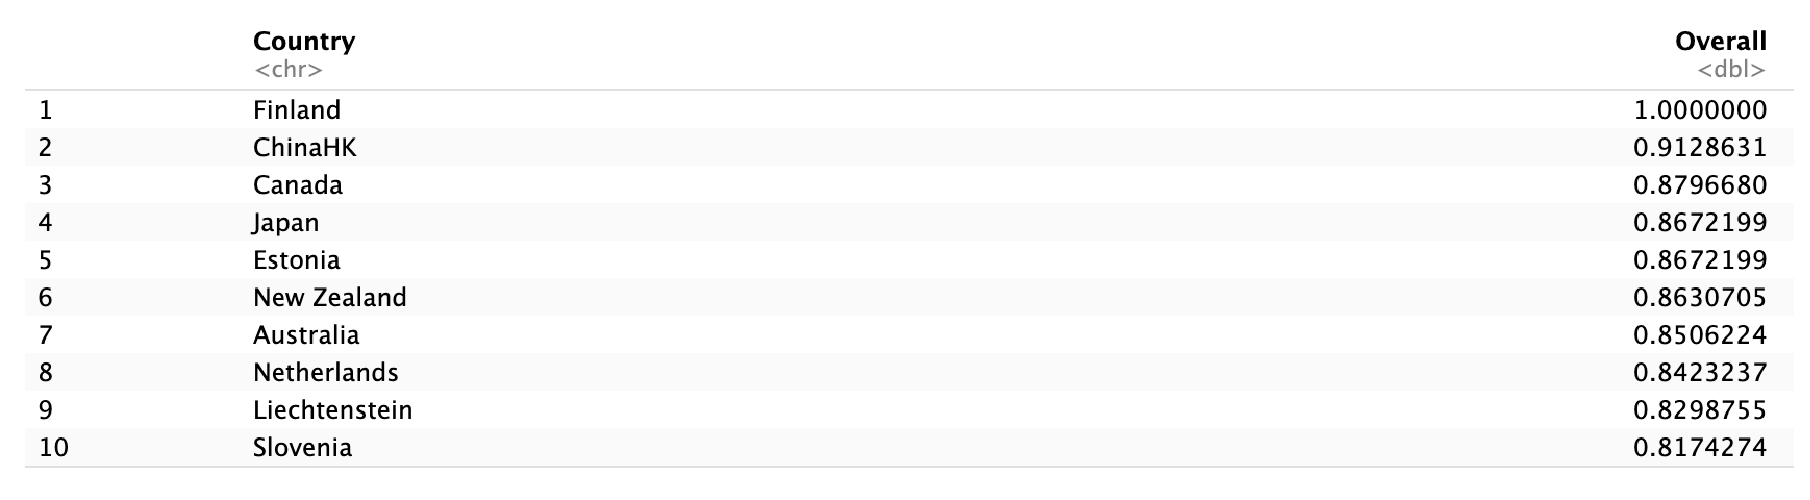
\includegraphics[width=\linewidth]{images/top10}
    \caption{TOP 10 Overall Countries}
    \label{fig:top10}
    \end{figure}

  \section{Statistical Models and Techniques Used}

  \subsection{Correlation Analysis}
  \label{ss.corr}
  
  Figure $\ref{fig:corr}$ presents the linear correlations among the variables. Notably:
  \begin{itemize}
  \item Income is negatively correlated with Support.
  \item HDI displays a negative correlation with Interest.
  \item Both Support and Interest are negatively correlated with the Overall Score.
  \end{itemize}
  
  \begin{figure}[htb]
  \centering
  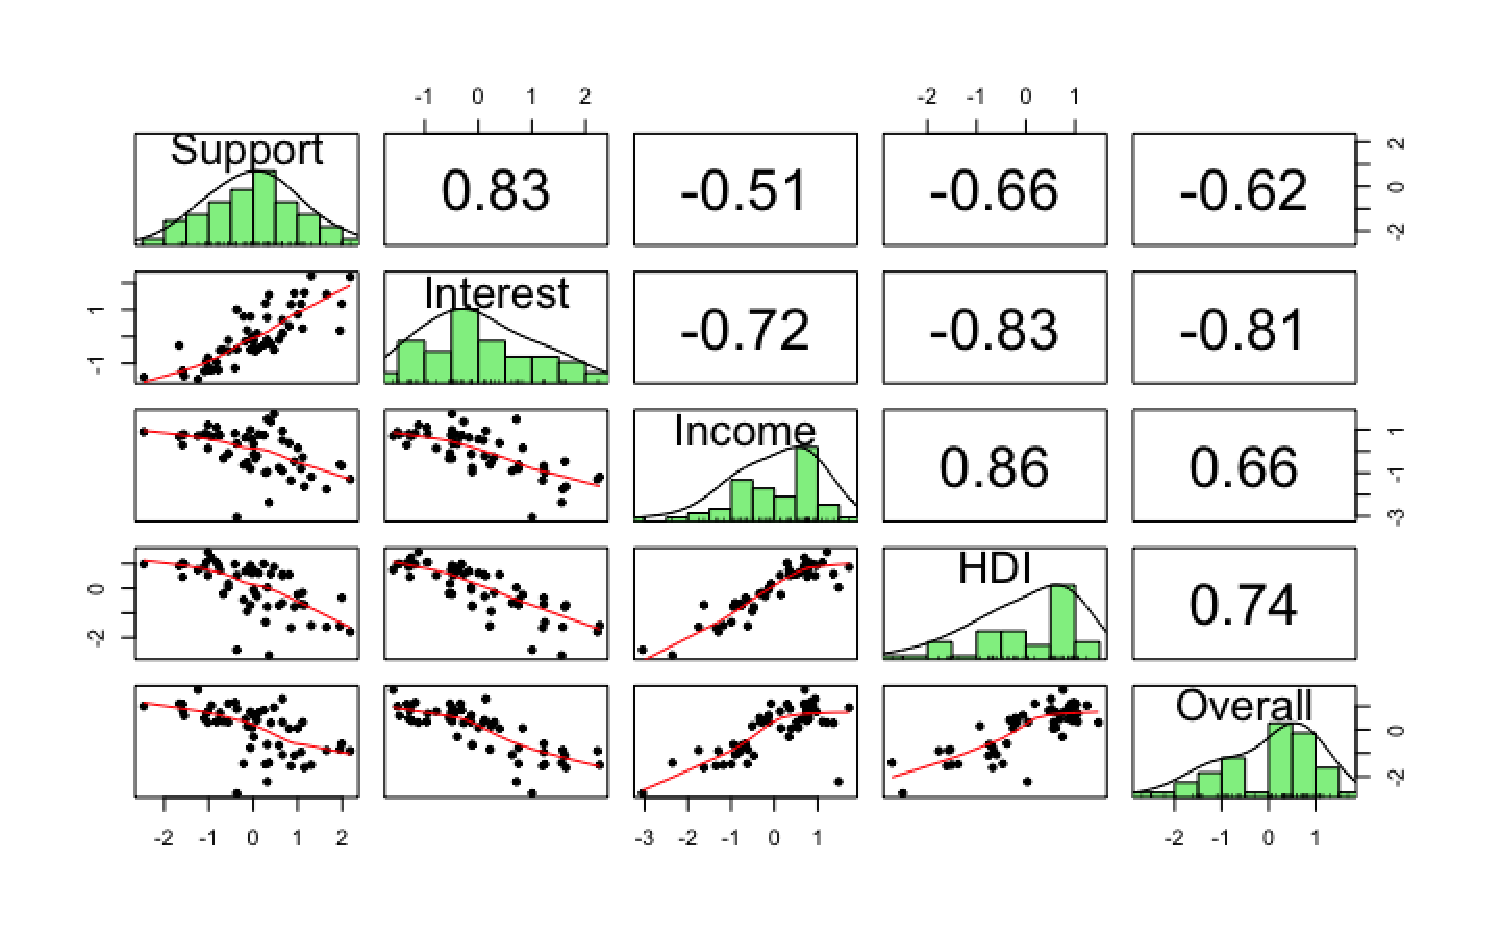
\includegraphics[width=\linewidth]{images/corr}
  \caption{Correlation Analysis of Variables}
  \label{fig:corr}
  \end{figure}
  
  \subsection{Regression Analysis}
  \label{ss.reg}
  
  \subsubsection{Relationship between Wealth and Support for Science}
  \label{sss.incvssup}
  
  We utilized linear regression to ascertain the relationship between a country's wealth (represented by Income) and its support for science. The model is expressed as:

$\text{Support} = -1.662 \times 10^{-16} - 0.4773 \times \text{Income} + \epsilon$

The model's $R^2$ value of 0.2278 suggests that approximately 22.78\% of the variance in Support is explained by Income. The adjusted $R^2$ is 0.213, providing a more nuanced measure of the model's fit.

The negative coefficient for Income implies that as income rises, support tends to decrease by 0.4773 units, all else being equal. The coefficient's statistical significance ($p-value < 0.05$) underscores the influence of income on support.

\subsubsection{Impact of HDI on Interest}
\label{sss.hdivsint}

To discern the influence of a country's HDI on its level of interest, we employed a simple linear regression:

$\text{Interest} = -9.748 \times 10^{-16} - 0.8163 \times \text{HDI} + \epsilon$

The coefficient for HDI, -0.8163, is statistically significant ($p-value < 0.05$). This suggests that as HDI increases, interest decreases by 0.8163 units, all else being constant. The model's $R^2$ value of 0.6663 indicates that HDI explains approximately 66.63\% of the variance in Interest.

\subsubsection{Influence of Support and Interest on Overall Score}
\label{sss.supintvsoverall}

To understand how Support and Interest influence the Overall Score, we used multiple linear regression:

$\text{Overall} = -1.445 \times 10^{-15} + 0.2502 \times \text{Support} - 0.9964 \times \text{Interest} + \epsilon$


The coefficient for Support, 0.2502, suggests a unit increase in Support corresponds to a 0.2502 unit increase in the Overall Score, with other factors held constant. However, its p-value of 0.07782 slightly exceeds the 0.05 threshold, indicating a potential relationship that isn't robustly significant.

Conversely, the coefficient for Interest, -0.9964, is statistically significant ($p-value < 0.05$), implying a unit increase in Interest leads to a decrease of 0.9964 units in the Overall Score, all else being constant.

The model's $R^2$ value of 0.6537 suggests that Support and Interest together explain approximately 65.37\% of the variance in the Overall Score.

\section{Key Findings}

Our statistical analyses, encompassing both correlation and regression, revealed linear relationships among the variables of interest. Specifically:

\begin{itemize}
\item HDI exerts a negative influence on Interest.
\item Income negatively impacts Support.
\item While Support positively affects the Overall Score, Interest has a detrimental effect on it.
\end{itemize}

Upon delving into a country-specific analysis with standardized variables:

\subsection{Income vs Support by Countries}

As depicted in Figure $\ref{fig:inc_sup}$, there isn't a significant difference in Support across countries, corroborating our earlier model that explained only 22% of the variance. However, the Netherlands stands out with an anomalous Support score when juxtaposed against the income trend at the country level.

\begin{figure}[htb]
\centering
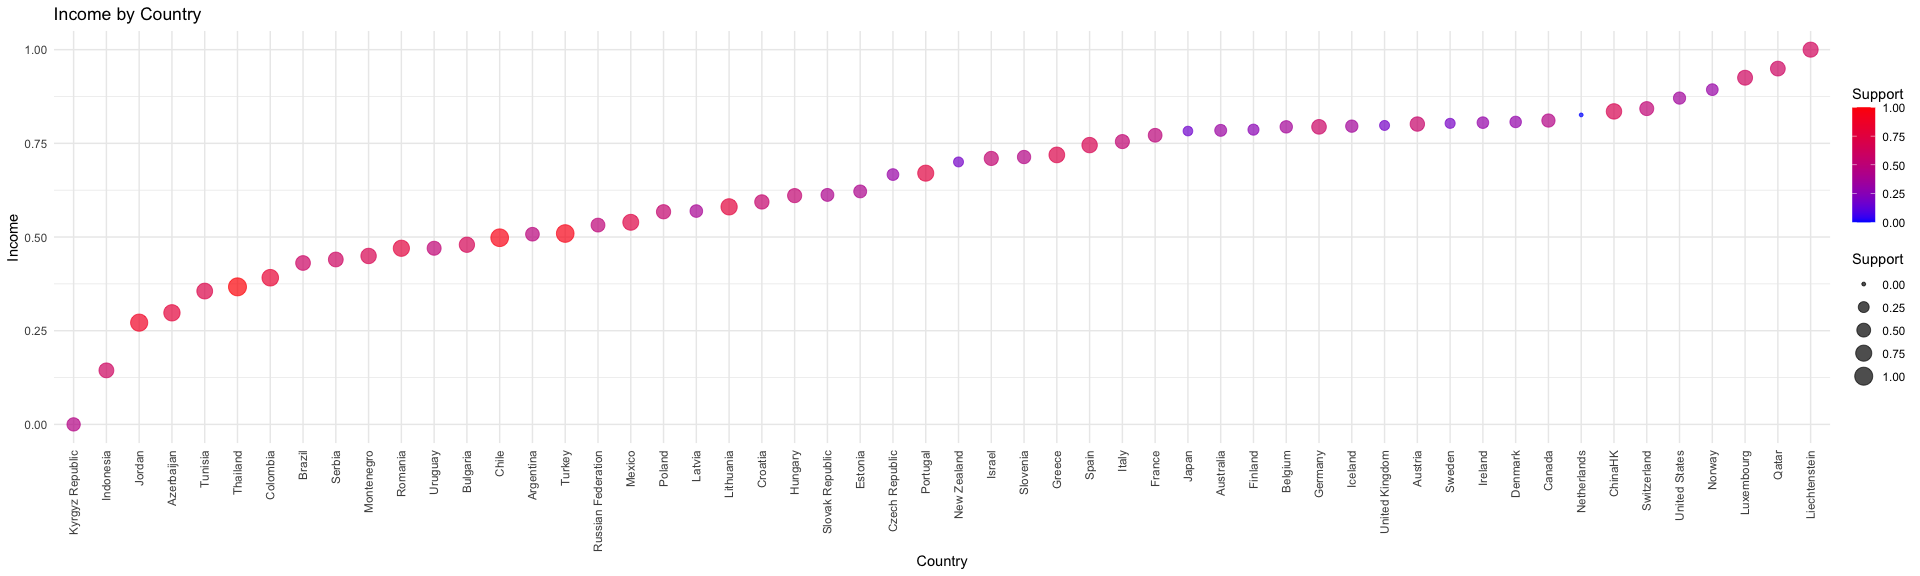
\includegraphics[width=\linewidth]{images/income_support_by_country}
\caption{Income vs Support by Countries}
\label{fig:inc_sup}
\end{figure}

\subsection{HDI vs Interest by Countries}

Figure $\ref{fig:hdi_int}$ illustrates that countries with a lower HDI tend to exhibit a heightened interest in Science. Yet, the United Kingdom and Finland deviate from this general trend, presenting unique patterns at the country level.

\begin{figure}[htb]
\centering
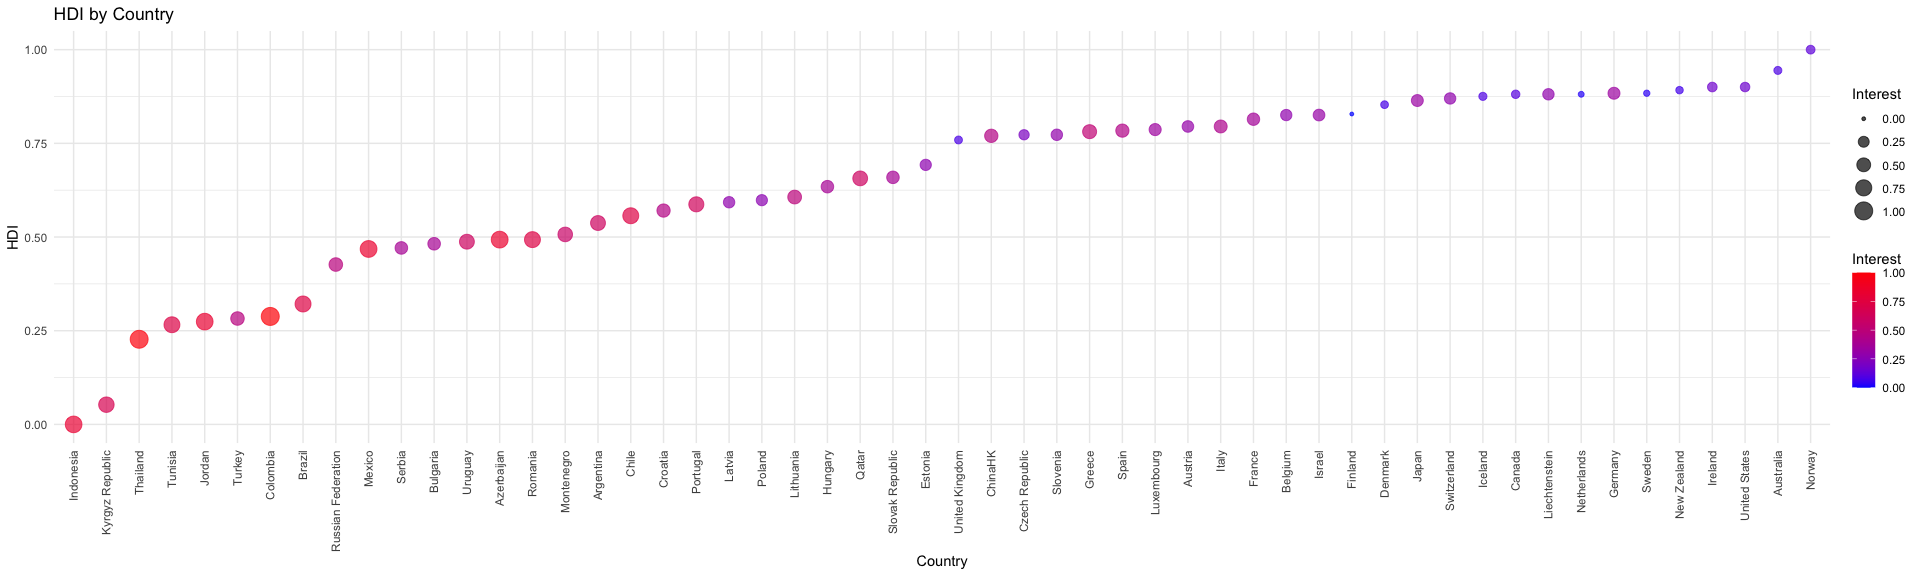
\includegraphics[width=\linewidth]{images/hdi_interest_by_country}
\caption{HDI vs Interest by Countries}
\label{fig:hdi_int}
\end{figure}

\subsection{Support and Interest vs Overall Score}

Figure $\ref{fig:int_sup_overall}$ indicates that lower Overall Scores predominantly fall within the range where 
$0.6 < Interest < 0.7$ and 
$0.4 < Support < 0.7$. 
Notably, both the Netherlands and Japan diverge from this trend, showcasing distinct patterns.

\begin{figure}[htb]
\centering
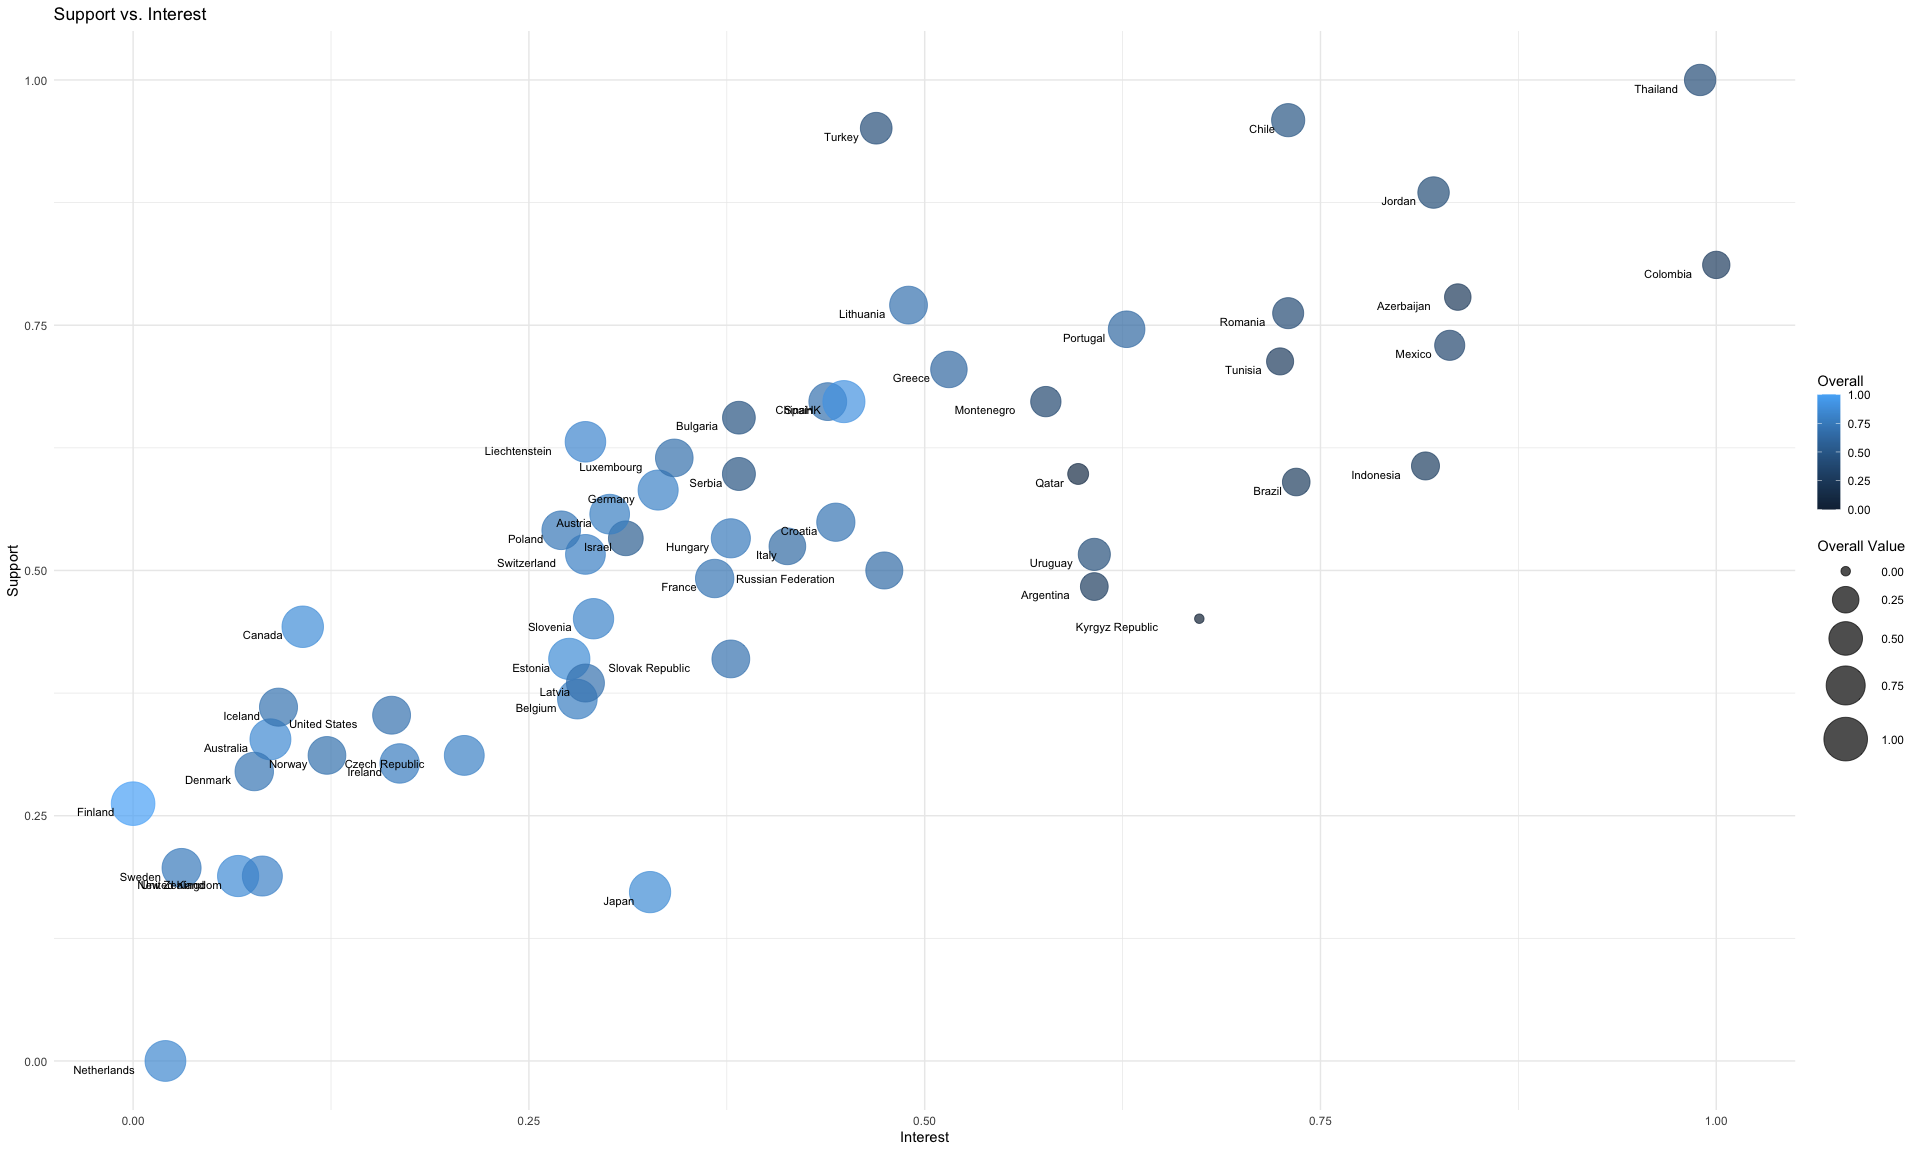
\includegraphics[width=\linewidth]{images/interest_support_vs_overall}
\caption{Support and Interest vs Overall Score by Countries}
\label{fig:int_sup_overall}
\end{figure}



\section{Recommendations and Future Research}

\subsection{Recommendations}

\begin{itemize}
\item \textbf{Netherlands:} Our analysis indicates that the support for science in the Netherlands is considerably lower compared to countries with similar income levels. We recommend that the Dutch government consider allocating additional funding to bolster science-related initiatives and programs. A deeper investigation may be warranted to pinpoint the underlying reasons for this discrepancy.

\item \textbf{Finland:} In comparison to nations with analogous Human Development levels, Finland exhibits a notably diminished interest in science among its students. It would be prudent for educational stakeholders in Finland to delve deeper into the root causes of this reduced interest. Initiatives aimed at reigniting students' passion for science might be beneficial.
\end{itemize}

\subsection{Future Research}

Future research endeavors could focus on:
\begin{itemize}
\item Conducting qualitative studies in countries like the Netherlands and Finland to gain insights into the specific factors affecting science support and interest, respectively.

\item Exploring the potential cultural, societal, or educational system differences that might influence students' attitudes towards science in various countries.

\item Investigating the role of external factors, such as media portrayal of science, in shaping students' perceptions and interests.
\end{itemize}

\section{Conclusions}

A prevailing assumption is that students hailing from affluent nations benefit from superior support in science and manifest a heightened interest in the subject. Contrary to this belief, our research, encompassing data from 54 countries, reveals that nations with lower Human Development Indices often exhibit a stronger interest in science. This suggests that the relative affluence and comfort experienced by students in wealthier countries might inadvertently dampen their curiosity and drive for scientific exploration.

The relationship between a country's income and its support for science also follows a similar trend, albeit the differences among countries aren't pronounced.

On a country-specific note, the Netherlands and Finland warrant special attention. The Netherlands, despite its economic stature, lags in science support when juxtaposed against its income counterparts. Conversely, Finland, despite its commendable Human Development standing, grapples with a diminished student interest in science. These findings underscore the intricate interplay of economic, developmental, and educational factors in shaping a nation's scientific landscape.

\newpage
%
%\bibliographystyle{harvard}
\bibliographystyle{apalike3}
%\bibliographystyle{abbrv} %this is the same as plainnat but with last name fist 
%\bibliographystyle{unsrtnat}  % Sets the bibliography style
                              % unsrtnat. See the article about
                              % bibliography styles for more
                              % information on
                              % https://www.sharelatex.com/learn/Natbib_bibliography_styles
\bibliography{BIBTEX_GOF} 


\end{document}


